\documentclass[pdftex,12pt,a4paper]{report}

\usepackage[pdftex]{graphicx}
\usepackage{float}
\usepackage{fancyvrb}
\fvset{xleftmargin=2em}
\usepackage{multicol}
\usepackage{wrapfig}

\usepackage{pgfplots}
\pgfplotsset{width=10cm,compat=1.9}
\usepackage{tikzscale}
\usepackage{pgfplotstable}
\usepackage{booktabs}
\usepackage[font=small,labelfont=bf,tableposition=top]{caption}

\usepackage[utf8]{inputenc} % isto é um comentário
\usepackage[portuges]{babel}
\usepackage[T1]{fontenc}
\usepackage{times}
%\usepackage{lmodern}
\usepackage[obeyspaces,spaces]{url}
\usepackage[left=25mm,right=25mm,top=25mm,bottom=25mm]{geometry}
\usepackage{titlesec}
\usepackage{mathtools}
%identa 1º paragrafo de capitulos e secções
\usepackage{indentfirst}

\newcommand{\HRule}{\rule{\linewidth}{0.5mm}}
\titleformat{\chapter}{\normalfont\huge}{\thechapter.}{20pt}{\huge}


\begin{document}

\begin{titlepage}


\begin{minipage}{0.3\textwidth}
\begin{flushleft} 

\includegraphics[width=\textwidth]{logo.png}
\end{flushleft}
\end{minipage}
\begin{minipage}{0.6\textwidth}
\begin{flushright} 

\textsc{Departamento de Engenharia Informática}\\[0.1cm]
\bfseries Mestrado Integrado em Engenharia Informática \\ [0.1cm]
\bfseries \textit{Programação Orientada aos Objetos}\\[8mm]

\end{flushright}
\end{minipage}


\vspace{3cm}


\begin{center}


\LARGE UMeR

\Large \textbf{\textit{Serviço de transporte de passageiros}}\\[1.5cm]


{\Large \bfseries Grupo XX\\[2cm] }


\noindent\begin{minipage}[b]{.2\textwidth}
	
\includegraphics[scale=0.18]{celia}
	\small{Célia Figueiredo a67637}
\end{minipage} 
\hfill
\begin{minipage}[b]{.2\textwidth}
	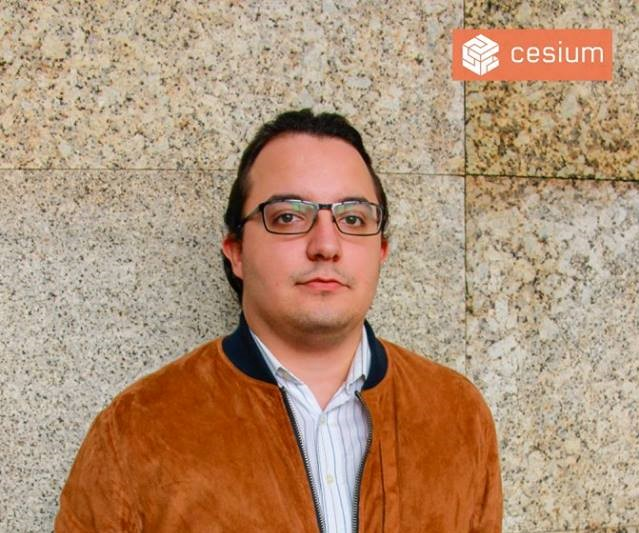
\includegraphics[scale=0.3]{luis}
	\small{José Carlos Faria a67638}
\end{minipage}
\hfill
\begin{minipage}[b]{.2\textwidth}
	
\includegraphics[scale=0.63]{nelson}
	\small{Márcia Costa a67672}
\end{minipage}




\vspace{3ex}


\vfill

\large Braga, {\large \today}

\end{center}
\end{titlepage}


\tableofcontents

\begin{abstract}

O presente relatório descreve o trabalho efetuado para a realização do projeto, onde foi pedido a implementação de um serviço de transporte de passageiros (UMeR) com o uso da linguagem \textit{JAVA} esta que é orientada aos objetos. 

\end{abstract}
\chapter{Introdução}
\label{cap:intro}

No âmbito da Unidade Curricular de Programação Orientada aos Objectos pertencente ao plano de estudos do 2º ano do Mestrado Integrado em Engenharia Informática foi proposto o desenvolvimento de um serviço de transporte de passageiros. 



\chapter{Descrição geral do projeto}
\section{UMeR}
Pretende-se que a aplicação a ser desenvolvida dê suporte a toda a funcionalidade que permita que um utilizador realize uma viagem num dos táxis da \textbf{UMeR}. O processo deve abranger todos os mecanismos de criação de utilizadores, motoristas, automóveis e posteriormente a marcação das viagens, a realização das mesmas e respectiva imputação do preço. Pretende-se também que o sistema guarde registo de todas as operações efectuadas e que depois tenha mecanismos para as disponibilizar (exemplo: viagens de um utilizador, extracto de viagens de um taxi num determinado período, valor facturado por um taxi num determinado período, etc.). 

Cada perfil de utilizador deve apenas conseguir aceder às informações e funcionalidades respectivas.

\begin{itemize}
	\item Os clientes dos táxis UMeR poderão:
	\begin{enumerate}
		\item solicitar uma viagem ao táxi mais próximo das suas coordenadas;
		\item solicitar uma viagem a um táxi específico;
		\item fazer uma reserva para um táxi específico que, de momento, não está disponível.
	\end{enumerate}
\end{itemize}

\begin{itemize}
	\item Os motoristas poderão:
	\begin{enumerate}
		\item sinalizar que estão disponíveis para serem requisitados;
		\item registar uma viagem para um determinado cliente;
		\item registar o preço que custou determinada viagem.
	\end{enumerate}
\end{itemize}

\subsection{Actores do sistema}

Existirão dois tipos distintos de actores no sistema, que partilham a seguinte informação:
\begin{itemize}
	\item email (que identifica o utilizador);
	\item nome;
	\item password;
	\item morada;
	\item data de nascimento.
\end{itemize}

\subsubsection{Cliente}
O Cliente representa a pessoa que solicita e efectua uma viagem de táxi. O cliente está sempre numa determinada localização (expressa em x e y, isto é, num espaço 2D) e escolhe um táxi específico ou então solicita o táxi mais perto que esteja disponível. O cliente tem também uma relação de todas as viagens que fez, com toda a informação relativa à viagem.

\subsubsection{Motorista - colaborador da UMeR}
O motorista conduz o táxi e além da informação atrás referida tem também dados relativos a: 
\begin{itemize}
	\item grau de cumprimento de horário estabelecido com o cliente, dado por um factor entre 0 e 100;
	\item classificação do motorista, dado numa escala de 0 a 100, calculada com base na classificação dada pelo cliente no final da viagem;
	\item histórico das viagens realizadas;
	\item número de kms já realizados na UMeR;
	\item informação sobre se está ou não disponível em determindado momento, isto é, se está ou não a trabalhar.
\end{itemize}

\subsection{Os táxis UMeR}

O ecossistema do UMeR contempla diferentes tipos de viaturas de aluguer (táxis). Neste momento estão em funcionamento os seguintes tipos de viaturas:

\begin{itemize}
	\item carros ligeiros;
	\item carrinhas de nove lugares;
	\item motos.
\end{itemize}
Cada um destes tipos de viaturas tem associada:
\begin{itemize}
	\item uma velocidade média por km;
	\item um preço base por km;
	\item um factor de fiabilidade, que determina a capacidade da viatura cumprir o tempo acordado com o cliente. Sempre que se realiza uma viagem é calculado (através da invocação de um random()) a capacidade de o veículo cumprir com o tempo acordado com o cliente. Este factor tem um efeito multiplicador sobre o tempo fornecido ao cliente.
\end{itemize}

Existem ainda alguns tipos de viaturas que possibilitam a existência de uma fila de espera de marcações. Quando o táxi não está disponível (por exemplo, pelo facto do condutor estar fora do horário de trabalho) é possível para essas viaturas aceitarem reservas de clientes. As reservas serão satisfeitas por ordem de chegada. Uma viatura sabe sempre a localização (em x e y) onde está. Quando realiza um serviço desloca-se para as coordenadas indicadas pelo cliente e fica aí parado até que seja solicitado um novo serviço.

\subsection{Fazer uma viagem no UMeR}
O processo de fazer uma viagem no UMeR segue as seguintes regras:
\begin{enumerate}
	\item o cliente indica as coordenadas x e y em que se encontra;
	\item o cliente decide se pretende chamar um táxi específico ou então solicitar o que está mais próximo;
	\item por uma questão de simplificação, os UMeR deslocam-se sempre em linha recta pelo que o cálculo da distância entre o cliente e o táxi é feito pela cálculo da distância euclidiana (exemplo: se o cliente estiver em (0,0) e o táxi em (2,2) a distância é de 2.8284 kms);
	\item após ser calculada a distância consegue-se saber, dadas as características do táxi, quanto tempo demora a chegar ao cliente e depois ao destino que o cliente solicita;
	\item o táxi indica ao cliente qual o custo estimado da viagem, tendo em conta o deslocamento que é necessário efectuar, e o tempo total de viagem;
	\item de acordo com a fiabilidade do carro (e de outros factores que pode considerar: a destreza do condutor, as condições metereológicas, etc.) é calculado o tempo real da viagem. Se a diferença for superior a 25\% do tempo estimado, então o preço a cobrar é o combinado com o cliente. Se a diferença for igual ou inferior a 25\% o valor é ajustado para o valor real em função do tempo decorrido;
	\item o táxi fica no ponto definido como fim da viagem à espera de nova solicitação de serviço;
	\item após a viagem o cliente pode dar uma nota ao motorista e fica com o documento relativo à viagem guardado na sua área pessoal.
\end{enumerate}

\subsection{Motoristas individuais vs Empresas de Táxi}
Numa primeira fase o UMeR foi pensado para condutores que conduziam a sua viatura e fazem serviço de transporte de clientes. No entanto, e devido ao sucesso do negócio, foram criadas empresas que possuem várias viaturas (em teoria de diversos tipos) e que empregam vários motoristas. A gestão que é feita destas empresas implica que após a criação da empresa se possam adicionar viaturas e motoristas, e que uma mesma viatura possa ser conduzida por motoristas diferentes (em tempos diferentes).

\subsection{Viaturas com Fila de Espera}
O UMeR possibilita que algumas viaturas possam ser definidas como possuindo uma fila de espera, que possibilita que quando a viatura está indisponível os pedidos sejam adicionados a uma fila de espera. Quando o veículo fica disponível são executadas todas as viagens inseridas na fila de espera, pela ordem de chegada. Os veículos com fila de espera possibilitam este comportamento, sendo que os demais não exibem este comportamento e nessa situação se a viatura estiver indisponível não será candidata a efectuar viagens.

\chapter{Conclusões e }

Aspetos a melhorar seriam a apresentação dos menus, poder-se-ia ter melhorado a organização, assim como o 

listar as funcionalidades ..... 
. as funcionalidade básicas da aplicação que foram implementadas 
existem fatores de aleatoriedade implemnetados para calcular o tempo real 
as filas de espera dos veiculos não podem ser utilizadas, 
não é possivel registar empresas. 
os menus poderiam ter uma melhor organização por exemplos as estaticias que são acedidas pelo admin devia ter um menu de introdução de estatisticas 

os motoristas deveriam poder criar vários veiculos e fazer a gestão do veiculo que estão a utilizar no momento. neste momento o motorista para reutilizar o veículo tem de o voltar a registar 

+/-não podem existir atores de tipos diferentes com o memso email, 

o admin deveria poder gerir clientes motoristas e veiculos 
neste momento só existe um admin e não tem a possibilidade de inserir outros admins 

não foi possivel u

Trabalho Futuro

Permitir registo de empresas e a utilização das filas de espera dos veiculos, para o primeiro ter-se-ia de adicionar um novo tipo de utilizador e dar-lhe permissão para conseguir gerir os seus motoristas e veiculos 

para o segundo seria necessário alterar a requisição de um motorista e  se ele permitisse fila de espera adicionar o cliente a essa fila e alterar o estado do cliente para em fila de espera. 

o admin deveria poder gerir clientes motoristas e veiculos





\end {document}


